\documentclass[12pt]{article}
\usepackage{geometry}
\usepackage{enumitem}
\usepackage[official]{eurosym}
\usepackage{graphicx}
\usepackage[utf8x]{inputenc}
\usepackage{float}
\usepackage{tabto}
\usepackage{hyperref}
\usepackage{subcaption}
\usepackage{placeins}
\usepackage{caption}

% There is a bug (Bug #1574052) with the titlesec package that causes the section 
% numbering to be missing. Fixed  are available online.
\usepackage{titlesec}


% Comment the following lines to use the default Computer Modern font
% instead of the Palatino font provided by the mathpazo package.
% Remove the 'osf' bit if you don't like the old style figures.
\usepackage[T1]{fontenc}
\usepackage[sc,osf]{mathpazo}

% Uncomment to disable hyphenation
%\usepackage[none]{hyphenat}

% Uncomment in case large amounts off overfull widthbox errors are given.
\setlength{\emergencystretch}{10pt}

\setlength{\parskip}{0pt}
\setlength{\parsep}{0pt}
\setlength{\headsep}{0pt}
\setlength{\topskip}{0pt}
\setlength{\topmargin}{0pt}
\setlength{\topsep}{0pt}
\setlength{\partopsep}{0pt}

% Control indentation
\setlength{\parindent}{0pt}

% Paragraph space
\setlength{\parskip}{11pt}

% Make lists without bullets
\newenvironment{itemize*}{
  \begin{list}{}{
    \setlength{\leftmargin}{1.5em}
  }
}{
  \end{list}
}

\hypersetup{
	linkcolor = black,
	colorlinks = true,
	urlcolor = black,
	pdfauthor = {Nukelawe},
	pdfpagemode = UseNone
}

\titleformat{\section}[block]{\Large}{\thesection}{1ex}{}
\titlespacing*{\section}{0cm}{0ex}{0cm}

\setenumerate{
	listparindent=\parindent,
	topsep=0pt,
	itemsep=0pt,
	partopsep=0pt
}
\setitemize{
	listparindent=\parindent,
	noitemsep,
	parsep=0pt,
	topsep=0pt,
	partopsep = 0pt
}

\geometry{
  body={6.5in, 8.5in},
  left=1.0in,
  top=1.25in
}

\graphicspath{ {images/} }
%\captionsetup{justification=raggedright,singlelinecheck=false}

\begin{document}
{\centering
{\huge Slime finder version 1.0}

{\Large by Nukelawe}\\
}
\vspace{2cm}
Slime finder is a command line java program to search for locations in a Minecraft world with specific amounts of slime chunks within certain range of a player. It was designed to look for mobfarm perimeter locations where the number of slime chunks in the perimeter is either very high or very low.

The program has two possible modes, search and image generation. They are both specified by giving command line arguments. The available options are the following:

\hspace{1.0cm}
\begin{tabular}{@{} l l l @{}}
\texttt{-h} & \texttt{-{}-help} & Shows the available options and their descriptions. \\
\texttt{-s} & \texttt{-{}-search} & Enters the search mode. \\
\texttt{-i} & \texttt{-{}-image} & Enters the image generation mode. \\
\end{tabular}

If both \texttt{-s} and \texttt{-i} are given the search will be performed first and the image generation immediately afterwards.

The settings for the slime finder are given in three separate property files. The files "\texttt{search.properties}" and "\texttt{image.properties}" contain settings for the search- and image generation modes, respectively and the file "\texttt{slime.properties}" contains general information that is needed in both modes.

\pagebreak
\section{\bfseries slime.properties}
The file "\texttt{slime.properties}" is used in both search and image generation modes and has the following fields:

\hspace{1.0cm}
\fbox{
\begin{tabular}{@{}l l@{}}
	\textbf{world-seed} & long\\ 
	\textbf{despawn-sphere} & boolean\\
	\textbf{exclusion-sphere} & boolean\\
	\textbf{eligible chunks} & boolean\\
	\textbf{y-offset} & integer\\
	\textbf{min-chunk-weight} & integer
\end{tabular}
}

\textbf{Block mask} at position P is the set of block positions with a particular y-coordinate in which a hostile mob could spawn if a player was positioned at P. Here we restrict ourselves to inspect a single y-coordinate because slime spawning depends heavily on altitude. 

The shape of the block mask is determined by the \textbf{y-offset} with respect to the player as well as the mask components listed below.
\begin{itemize}[label={},leftmargin=1cm]
\item \textbf{Despawn sphere} is a sphere of radius 128 blocks centered around a player outside which a slime would instantly despawn.
\item \textbf{Exclusion sphere} is a sphere of radius 24 centered around a player inside which mobs cannot spawn.
\item \textbf{Eligible chunks} are the chunks in a 15$\times$15-chunk square centered around a chunk a player is in. These are the chunks in which the natural mob spawner attempts to spawn mobs.
\end{itemize}
Each of the mask components can be individually disabled in the "\texttt{slime.properties}"-file by setting them to false. How the block mask is calculated from the mask components is illustrated in figure \ref{fig:block-mask-components}.

\begin{figure}[H]
\begin{subfigure}{0.25\textwidth}
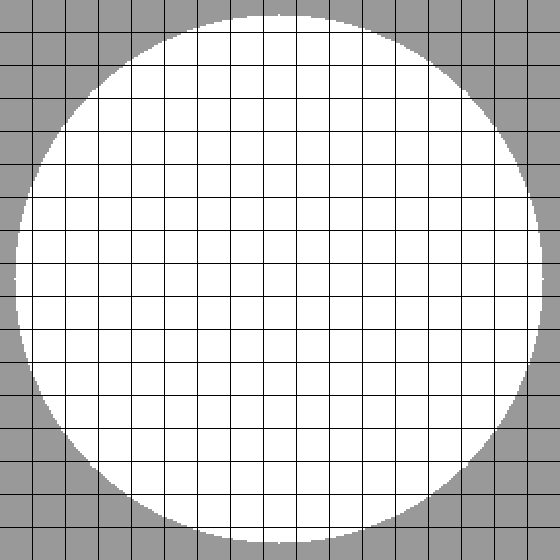
\includegraphics[width=.9\linewidth]{despawn-sphere.png}
\caption{Despawn sphere}
\label{fig:despawn-sphere}
\end{subfigure}%
\begin{subfigure}{0.25\textwidth}
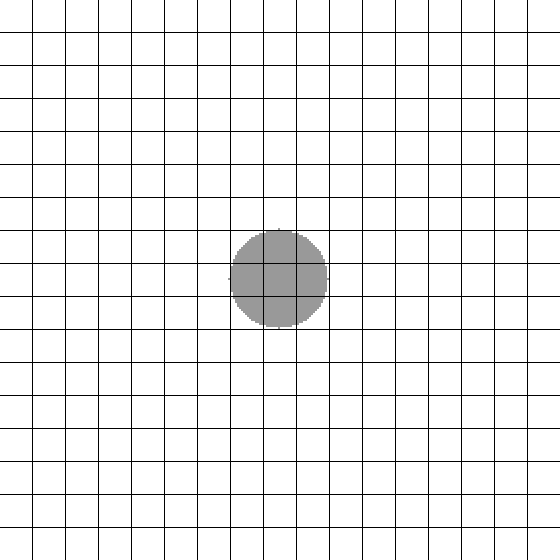
\includegraphics[width=.9\linewidth]{exclusion-sphere.png}
\caption{Exclusion sphere}
\label{fig:exclusion-sphere}
\end{subfigure}%
\begin{subfigure}{0.25\textwidth}
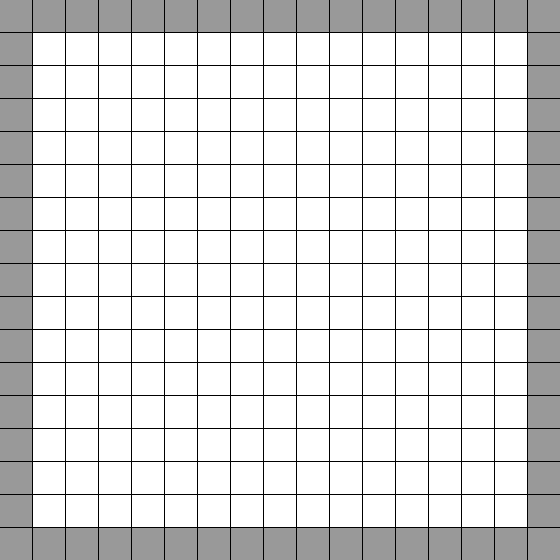
\includegraphics[width=.9\linewidth]{eligible-chunks.png}
\caption{Eligible chunks}
\label{fig:eligible-chunks}
\end{subfigure}%
\begin{subfigure}{0.25\textwidth}
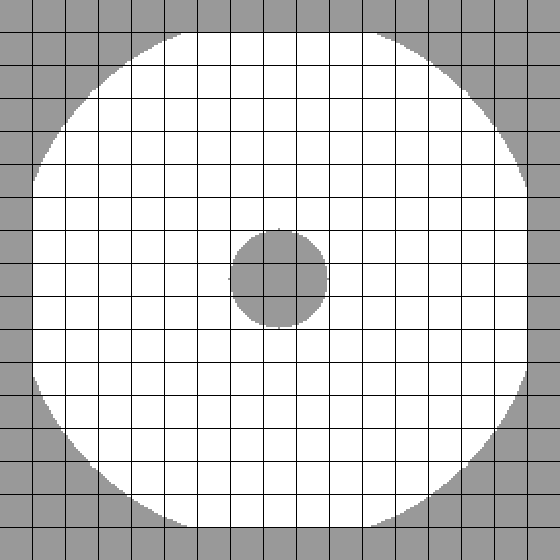
\includegraphics[width=.9\linewidth]{block-mask.png}
\caption{Block mask}
\label{fig:block-mask}
\end{subfigure}
\caption{Components of a block mask with y-offset $= 0$}
\label{fig:block-mask-components}
\end{figure}

{\bfseries Chunk mask} at position P is the set of chunks for which the number of blocks inside the corresponding block mask is greater than or equal to {\bfseries min-chunk-weight}. How the chunk mask depends on the min-chunk-weight is illustrated in figure \ref{fig:chunk-mask}.

\begin{figure}[H]
\begin{subfigure}{0.5\textwidth}
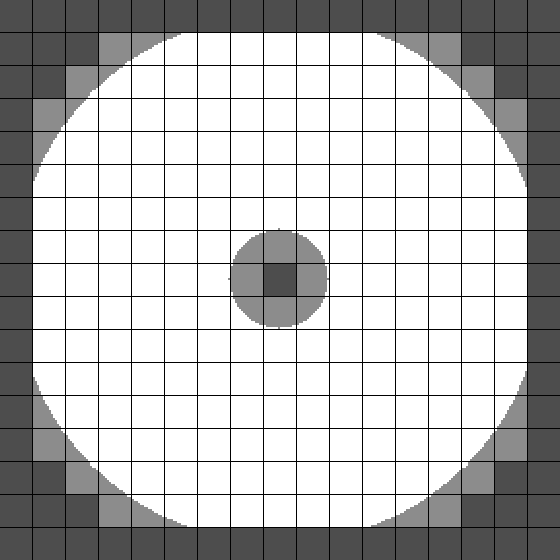
\includegraphics[width=.9\linewidth]{min-chunk-weight=1.png}
\captionsetup{width=.8\linewidth}
\caption*{\textbf{min-chunk-weight} = 1\\
At least one block in each chunk is contained by the block mask.}
\end{subfigure}%
\begin{subfigure}{0.5\textwidth}
\centering
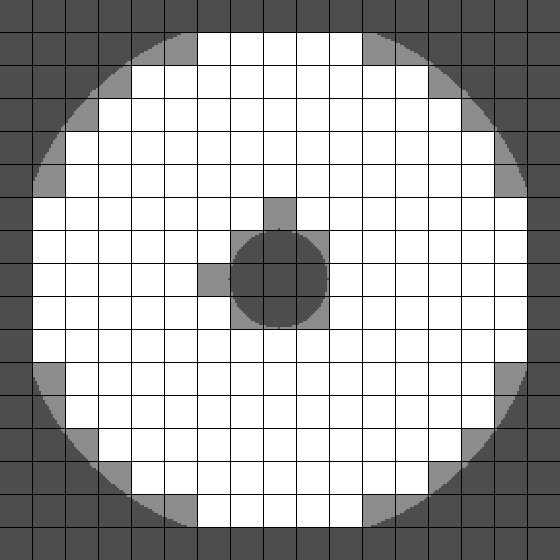
\includegraphics[width=.9\linewidth]{min-chunk-weight=256.png}
\captionsetup{width=.8\linewidth}
\caption*{\textbf{min-chunk-weight} = 256\\
Chunks are completely contained by the block mask.}
\end{subfigure}
\caption{Effect of min-chunk-weight on the chunk mask}
\label{fig:chunk-mask}
\end{figure}

\pagebreak
\section{\textbf{search.properties}}
\label{search.properties}
The file "\texttt{search.properties}" is used in the search mode and has the following fields:

\hspace{1.0cm}
\fbox{
\begin{tabular}{@{}l l@{}}
	\textbf{output-file} & string\\ 
	\textbf{append} & boolean\\
	\textbf{pos-block} & coordinate\\
	\textbf{pos-chunk} & coordinate\\
	\textbf{pos-in} & coordinate\\
	\textbf{min-width} & integer\\
	\textbf{max-width} & integer\\
	\textbf{fine-search} & boolean\\
	\textbf{min-block-size} & integer\\
	\textbf{max-block-size} & integer\\
	\textbf{min-chunk-size} & integer\\
	\textbf{max-chunk-size} & integer
\end{tabular}
}

\textbf{Block size} and \textbf{chunk size} are the numbers of slime chunks within the block mask and the chunk mask, respectively. Block size can be a fraction as a chunk can be only partially inside the block mask.

In the search mode the slime finder looks for positions for which block size and chunk size are within a range specified by the properties \textbf{min-block-size} and \textbf{max-block-size} for the block size and \textbf{min-chunk-size} and \textbf{max-chunk-size} for the chunk size.\\
If criteria for either chunk or block size is omitted every value will be matched.\\
If both criteria are given results matching either one will be recorded.

A starting position for the search is given either by specifying a block position in the \textbf{pos-block}-field or a chunk position and a within-chunk position in the \textbf{pos-chunk} and \textbf{pos-in}-fields respectively. All coordinates are given in the format \texttt{x,z}, where \texttt{x} and \texttt{z} are both integers.

The search will check all chunk positions in the square of width \textbf{max-width} centered around the starting chunk. Positions in the square of width \textbf{min-width} centered around the starting chunk are skipped.
The positions will be iterated through in a spiralling manner which ensures that matches are listed from closest to farthest from starting position.

If \textbf{fine-search} option is set to true all block positions in each chunk are checked. Otherwise only one position within each chunk is checked.

The matching positions found are written to the console and on a file specified by the \textbf{output-file}-field. If the file does not exist a new one with the given name will be created if possible. Unless \textbf{append} is set to true an existing output file will be overwritten without a warning! The output-file-field can also contain a path to a directory.

Every line in the output file containing no data should either start with a \texttt{\#} or consist of whitespace only. This is important for the file to be readable when used as an input for the image generation mode. 

Lines of data are formatted as follows:

\begin{center}
\texttt{%
\begin{tabular}{@{}l l l l l@{}}
blockPos & chunkPos & blockSize & chunkSize & extrema \\
x,z & xchunk:xin,zchunk:zin & size/area & size/area & 
\end{tabular}
}
\end{center}

Where \texttt{x} and \texttt{z} are block coordinates,\\
\texttt{xChunk} and \texttt{zChunk} are chunk coordinates,\\
\texttt{xIn} and \texttt{zIn} are block coordinates within the chunk,\\
\texttt{area} are the total numbers of chunks in the masks.\\
The extrema field indicates if the position has a minimum or maximum block or chunk size position among the positions checked so far.

\pagebreak
\section{\bfseries image.properties}
The file "\texttt{image.properties}" is used in the image generation mode and has the following fields:

\hspace{1.0cm}
\fbox{
\begin{tabular}{@{}l l@{}}
	\textbf{input-file} & string\\ 
	\textbf{output-dir} & string\\
	\textbf{block-width} & integer\\
	\textbf{grid-width} & integer\\
	\textbf{draw-slime-chunks} & boolean\\
	\textbf{draw-block-mask} & boolean\\
	\textbf{draw-chunk-mask} & boolean\\
	\textbf{draw-center-block} & boolean
\end{tabular}
}

\textbf{input-file} is the name of the file where positions to be generated into images will read from. This file should be formatted as specified in section \ref{search.properties}.

\textbf{output-dir} is the directory where the generated images will be placed. If the directory does not exist a new one will be created.

\textbf{block-width} and \textbf{grid-width} are the widths of a block and a gridline in pixels.

\textbf{draw-slime-chunks}, \textbf{draw-block-mask}, \textbf{draw-chunk-mask} and \textbf{draw-center-block} determine what features will be drawn on the image.




\end{document}
